\section{Metodología}
Para la realización del Trabajo Terminal se utilizará la metodología SCRUM ya que es una metodología ágil y que es altamente flexible, ya que la lista de sprints pueden ser modificadas en el transcurso del desarrollo del proyecto por diversos motivos que se tengan. Otro punto de SCRUM es que al trabajar por partes pequeñas y comenzar por las más importantes, es más fácil poder detectar problemas a futuro que tal vez puedan presentarse\cite{Referencia13}.

''Scrum es un proceso en el que se aplican de manera regular un conjunto de buenas prácticas para trabajar colaborativamente, en equipo, y obtener el mejor resultado posible de un proyecto. Estas prácticas se apoyan unas a otras y su selección tiene origen en un estudio de la manera de trabajar de equipos altamente productivos."\cite{Referencia14}

Uno de los beneficios de la metodología SCRUM es que los proyectos pueden ser entregados con una mejor calidad, ya que como es más fácil detectar problemas, estos pueden ser corregidos en el momento justo, antes de que seán más costosos y difíciles de corregir. 

En la figura \ref{fig:metodologiaSCRUM} se muestran las principales actividades abordadas por la metodología Scrum.
\newpage
\begin{figure}[htb]
	\centering
	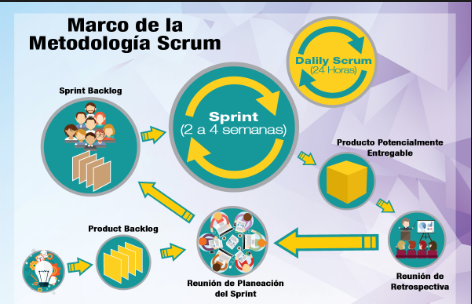
\includegraphics[width=1\textwidth]{images/introduccion/scrum}
	\caption{Marco de la Metodología SCRUM} \label{fig:metodologiaSCRUM}
\end{figure}

Se tendrán además prototipos de desarrollo donde se llevarán a cabo el análisis, diseño, construcción y pruebas de los prototipos implementados en cada etapa de la metodología anteriormente mencionada.

Esta metodología será aplicada a nuestro Trabajo Terminal de la siguiente manera:\\

\textbf{Trabajo Terminal 1}
\begin{itemize}
	\item Se trabajarán los primeros 2 sprints para esta primer parte del Trabajo Terminal.
	\item El sprint 1 constará del análisis de requerimientos, análisis del proceso y el análisis formal del Trabajo Terminal por medio de casos de uso. Para el trabajo terminal 1, solamente se hará el análisis formal del rol del Paciente por medio de casos de uso.
	\item El sprint 2 constará del diseño del sistema, diseño de pantallas por medio de mockups e implementación del primer prototipo que en este caso, será únicamente la parte del rol del \textbf{Paciente.}
\end{itemize}

\textbf{Trabajo Terminal 2}
\begin{itemize}
	\item Se trabajarán los últimos 3 sprints para esta segunda parte del Trabajo Terminal.
	\item El sprint 3 constará de la definición formal de la aplicación.
	\item El sprint 4 constará del diseño del sistema, diseño de pantallas por medio de mockups e implementación de los prototipos restantes que en este caso, serán las partes de los roles del \textbf{Doctor} y el \textbf{Auxiliar}.
	\item El sprint 5 constará de las pruebas de la aplicación, la generación del manual de usuario y la generación del reporte técnico para la entrega final del Trabajo Terminal.
\end{itemize}


\section{Arquitectura}

En la figura \ref{fig:arquitectura} se muestra el diagrama de la arquitectura propuesta con la que se trabajará para solucionar la problemática.

%En la figura \ref{fig:arquitectura} se describirá la arquitectura propuesta para la solución de la problemática.

\begin{figure}[htb]
	\centering
	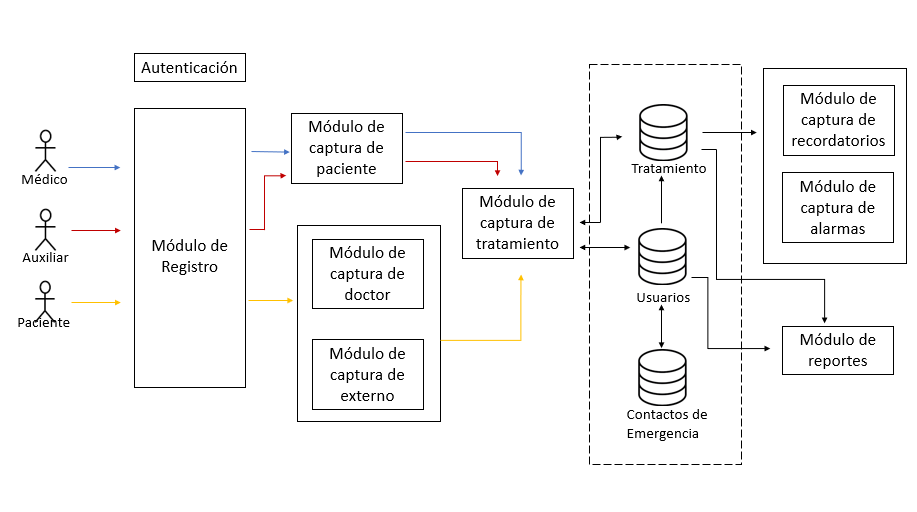
\includegraphics[width=1\textwidth]{images/cap2/Arquitectura}
	\caption{Arquitectura} \label{fig:arquitectura}
\end{figure}

Como podemos notar en la figura \ref{fig:arquitectura} se cuenta con tres roles que participarán en el sistema, los cuales son :
\begin{itemize}

	\item Paciente: Se le llama paciente a la persona que cuenta con un tratamiento generado por el médico que se encuentra a cargo de su salud.\\
	
	Las acciones con las que cuenta su rol son:
	\begin{itemize}
		\item Consultar sus tratamientos médicos.
		\item Agregar el tratamiento médico.
		\item Agregar medicina a tratamiento médico.
%		\item Modificar el tratamiento médico.
%		\item Eliminar el tratamiento médico.
		\item Agregar doctor
		\item Consultar doctor.
%		\item Asociar doctor.
		\item Eliminar doctor.
		\item Agregar auxiliar
		\item Consultar auxiliares.
%		\item Asociar auxiliar.
		\item Eliminar auxiliar.
		\item Agregar contactos de emergencia
		\item Consultar contactos de emergencia.
%		\item Asociar contacto de emergencia.
		\item Eliminar contacto de emergencia.
%		\item Editar recordatorios.
		\item Consultar recordatorios.
		\item Consultar alarmas.
		\item Consultar sus datos.
		\item Editar sus datos.
	\end{itemize}

	\item Doctor: \textbf{Doctor} dentro del sistema es el profesional de la salud que se encarga del diagnóstico del paciente.
	Las acciones con las que cuenta su rol son:
		\begin{itemize}
			
			\item Consultar pacientes.
			\item Consultar tratamiento de pacientes.
			\item Modificar tratamiento de pacientes.
			\item Eliminar tratamiento médico de sus pacientes.
			\item Agregar paciente nuevo.
%			\item Asociar nuevo paciente.
			\item Agregar tratamiento.
			\item Agregar medicina a tratamiento médico.
%			\item Editar notificaciones.
			\item Consultar historial clínico.
			\item Eliminar paciente.
			\item Editar paciente.
			
		\end{itemize}

	\item Auxiliar: nace de la necesidad de ayudar a los pacientes que cuentan con poca o nula experiencia los dispositivos móviles o que por factores ajenos a la aplicación como son la edad o alguna enfermedad, les sea imposible utilizar la aplicación por si mismos\\
	Las acciones con las que cuenta su rol son:
	\begin{itemize}
		
		
		\item Agregar paciente.
		\item Eliminar paciente.
		\item Editar paciente.
		\item Consultar tratamiento de paciente.
		\item Agregar tratamiento de paciente.
		\item Agregar medicina a tratamiento médico.
%		\item Modifica tratamientos.
		\item Eliminar tratamiento de paciente.
%		\item Editar sus notificaciones.
		\item Agregar doctor
		\item Consultar doctor.
		\item Eliminar doctor
%		\item Asociar doctor.
		\item Agregar contactos de emergencia
		\item Consultar contactos de emergencia.
		\item Eliminar contacto de emergencia.
		\item Consultar recordatorios.
		\item Consultar alarmas.
%		
%		\item Agregar Paciente.
%		\item Modificar Paciente.
%		\item Eliminar Paciente.
%		\item Agregar Tratamiento medico.
%		\item Modificar Tratamiento medico.
%		\item Consultar Tratamiento medico.
%		\item Modificar notificación
	\end{itemize}
\end{itemize}


\section{Módulos}
La arquitectura contará con los siguientes módulos:
\begin{itemize}
	\item Módulo de Registro: Este módulo es el encargado de registrar e ingresar a los actores dentro de la aplicación. 
	
	
	\item Módulo de Autenticación: Una vez que te hayas registrado dentro de la aplicación, el módulo de autenticación se encargará de verificar tu usuario y habilitar los módulos correspondientes a tu rol.
	
	\item Módulo de Inicio de Sesión: Este módulo te permitirá ingresar a los módulos correspondientes a tu rol ingresando con tu usuario y contraseña previamente registrados e el Módulo de Registro.
	
	 
	\item Módulo de Captura de Paciente: Este módulo es el encargado de agregar al paciente con el que trabajarán el doctor y el auxiliar.
	
	\item Módulo de Captura de Doctor: Este módulo es el encargado de agregar al doctor que está a cargo del tratamiento del paciente.
	
	\item Módulo de Captura de Auxiliar: Este módulo es el encargado de agregar al auxiliar que está a cargo del tratamiento del paciente.
	
	\item Módulo de Captura de Contactos de Emergencia:Este módulo es el encargado de agregar los contactos de emergencia que podrán recibir las alertas del paciente que los haya agregado.
	
	\item Módulo de Captura de Tratamiento: Este módulo es el encargado de ingresar el tratamiento médico del paciente y con el que podrán trabajar tanto el doctor como el auxiliar. 
%	y lo asociara al perfil del paciente con la información correspondiente del tratamiento.

	\item Módulo de Captura de Medicamentos: Este módulo es el encargado de ingresar los medicamentos que son recetados por el Doctor para que el paciente siga su tratamiento médico.
	
	\item Módulo de Recordatorios: Este módulo es el encargado de crear los recordatorios de las medicinas una vez que éstas hayan sido ingresadas dentro del tratamiento médico.
	
	\item Módulo de Alarmas: Este módulo es el encargado de crear las alarmas cuando un medicamento sea de alta prioridad y que si no se toma en el momento, pueda tener efectos negativos en el paciente.
	
	\item Módulo de Reportes: Este módulo es el encargado de generar un reporte con la información del tratamiento y datos relevantes del paciente como lo son la edad, estatura, peso, etc.
	
	
	
	
	
%	\item Módulo de Autenticación: El modulo encargado de verificar tu perfil y darte acceso a los módulos correspondientes.
%	\item Módulo captura de tratamientos: El modulo encargado de ingresar el tratamiento medico y lo asociara al perfil del paciente con la información correspondiente del tratamiento.
%	\item Módulo de recordatorios: Una vez que se paso por el modulo de \textbf{Captura de tratamiento} llegamos al modulo de recordatorios en donde se generaran los notificaciones a partir de la información obtenida del modulo de captura de tratamiento.
%	\item Módulo de alarmas: Este modulo es el encargado de cuando una notificación no haya sido silenciada esta se convierta en una alarma que le estará recordando al paciente tomar su medicamento.
%	\item Módulo de reportes: El modulo de reportes sirve para notificar al medico y al paciente que tan constante ha sido con su tratamiento.
%	\item Módulo de estadísticas: 
\end{itemize}

\section{Modelo Relacional}
En la siguiente figura \ref{fig:modelorelacional} se muestra el modelo relacional con el que trabajará la aplicación mostrando así los datos que estarán proporcionando cada una de las partes responsables para que funcionen de manera correcta todos los módulos.
\begin{figure}[htb]
	\centering
	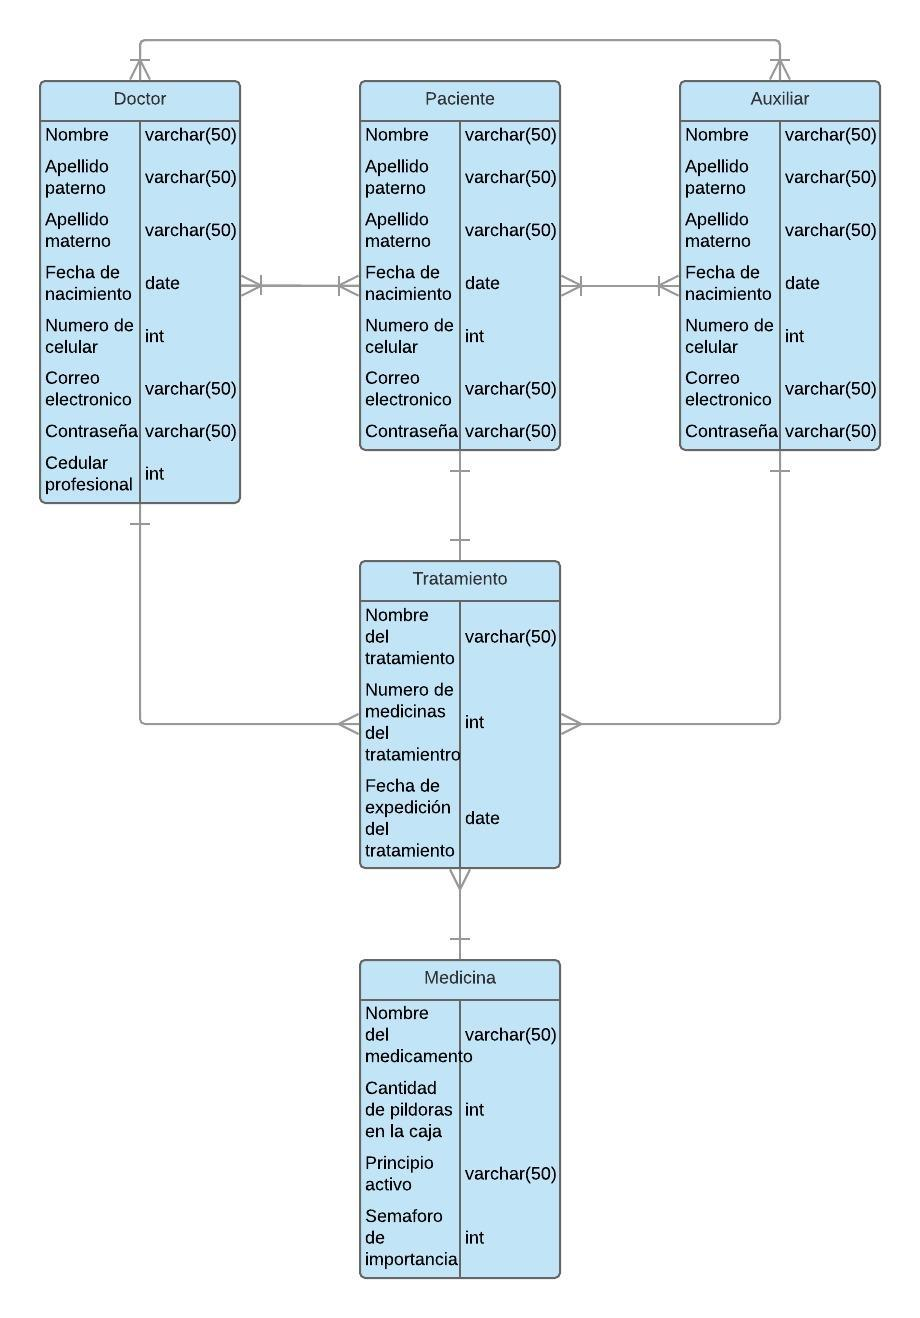
\includegraphics[width=1.1\textwidth]{images/cap2/modelorelacional}
	\caption{Modelo Relacional de Rem-Pills} \label{fig:modelorelacional}
\end{figure} 




\section{Requerimientos}
Los requerimientos funcionales describen lo que el sistema debe hacer. Son declaraciones de los servicios que debe proporcionar el sistema, de la manera en que éste debe reaccionar a entradas particulares y de cómo se debe comportar en situaciones particulares.\\
En la siguiente sección se especificarán los requerimientos con los que estará trabajando la aplicación.\\
%\begin{itemize}
%		\item RF1 - Registro de Usuario
%		La aplicación permitirá el registro de nuevos usuarios mediante el ingreso de su nombre, correo electrónico y contraseña.
%		
%		\item RF2 - Acceso al Sistema.
%		La aplicación permitira el acceso al sistema proporcionando el correo electrónico y la contraseña con la que se registraron en la aplicación
%		
%		Los usuarios accederán al sistema proporcionando el correo electrónico y la contraseña con la que se registraron en la aplicación
%		
%		\item RF3 - Agregar Paciente.
%		 
%		 La aplicación permitirá que tanto el doctor como el auxiliar agreguen a los pacientes con los que están trabajando a la \textbf{lista de pacientes}.
%		 
%		El usuario doctor agregará a un paciente a su \textbf{lista de pacientes} ingresando el correo electrónico o nombre del paciente.
%		El usuario auxiliar agregará a un paciente a su \textbf{lista de pacientes} ingresando el correo electrónico o nombre del paciente.
%		El usuario paciente agregará a un doctor a su \textbf{lista de doctores} ingresando el correo electrónico o nombre del paciente.
%		El usuario paciente agregará a un doctor a su \textbf{lista de auxiliares} ingresando el correo electrónico o nombre del paciente.
%	
%		\item RF4 - Agregar Doctor o Auxiliar.
%		
%		La aplicación permitirá al Paciente agregar al doctor que receto su tratamiento a su \textbf{lista de doctores} y en el caso de que sea necesario, agregar a la \textbf{lista de auxiliares} a un auxiliar para que sea el encargado de su tratamiento.
%		
%%		\item RF5 - Alta de Invitación.
%%		
%%		Cuando un usuario haya agregado a otro usuario, la aplicación mandará un correo con el cual se vincularán sus perfiles.
%		
%		\item RF6 - Agregar Tratamiento.
%		
%		La aplicación permitirá  ya sea al doctor, auxiliar o paciente agregar el tratamiento expedido por el doctor al perfil del paciente en cuestión.
%		
%		\item RF7 - Creación de Recordatorios.
%		
%		La aplicación creará los recordatorios de los medicamentos a tomar  una vez que el tratamiento haya sido ingresado en el sistema.
%		
%		\item RF8 - Creación de Alarmas.
%		
%		La aplicación permitirá al usuario configurar alarmas cuando el ingerir un medicamento sea de suma importancia.
%		
%		\item RF9 - Gestión de Contactos de Emergencia.
%		
%		Cuando una notificación de un medicamento con un alta importancia no haya sido silenciada después de tres intentos, la aplicación mandará un mensaje a los contactos de emergencia.
%		
%		\item RF10 - Creación de reportes.
%		
%		La aplicación permitirá al usuario ingresar datos relevantes de su salud y creará un reporte con el avance de sus tratamientos los datos ingresados.
%\end{itemize}
%
%
%Requerimientos No Funcionales
%\begin{itemize}
%	\item RNF-1 Creación de Usuario
%	La creación del usuario dependerá del rol que tenga, esto quiere decir que el formulario que llenará un doctor es distinto al de un paciente.
%	
%	\item RNF-2 Verificación de Perfil
%	La aplicación distinguirá entre los 4 tipos de roles que hay, los cuales son: Paciente, Auxiliar, Doctor y Administrador.
%	
%	\item RNF-3 Recordatorios.
%	Un recordatorio esta compuesto por un mensaje que se desplegara en la pantalla y que al llegar generara un sonido, notificando que es tiempo de tomar el medicamento.
%	
%	\item RNF-4 Interfaz Comprensible.
%	La aplicación contará con iconos, botones y formularios que muestran de forma clara lo que hace cada uno y con datos que se consiguen de la receta que expide el medico o que viene en la caja del medicamento.
%	
%	\item RNF-5 Base de datos.
%	La aplicación contará con una base de datos de forma local que permitirá que la consulta de los datos sea más rápida.
%	
%	\item RNF-6 Desarrollo Multiplataforma.
%	La aplicación sera desarrollada para los sistemas operativos iOS y Android de forma nativa permitiendo así explotar todas sus ventajas.
%	
%	\item RNF-7 Desempeño Web y Móvil.
%	La aplicación permitirá que el registro del tratamiento sea ingresado por una servicio web o mediante la aplicación móvil. 
%	
%	\item RNF-8	Protección de Información
%	La aplicación contará con un cifrado AES-128 para proporcionar toda la seguridad a la información del usuario.
%\end{itemize}





	
	
	\begin{ReqUser}		
		\reqUserItem{RF1}{Registro de Usuario}{
			El usuario requiere de un mecanismo que le permita registrarse en la aplicación.
		}
		{\alta}{}{\corregir}
	\end{ReqUser}
	\newpage
	\begin{ReqUser}		
		\reqUserItem{RF2}{Acceso al Sistema}{
			El usuario requiere de un mecanismo que le permita ingresar al sistema.
		}
		{\alta}{}{\corregir}
	\end{ReqUser}


	\begin{ReqUser}		
		\reqUserItem{RF3}{Recuperar Contraseña}{
			El usuario requiere de un mecanismo que le permita recuperar su contraseña o crear una contraseña nueva.
		}
		{\alta}{}{\corregir}
	\end{ReqUser}

	\begin{ReqUser}		
		\reqUserItem{RF4}{Agregar Paciente}{
			El doctor y el auxiliar requieren de un mecanismo que le permita agregar a un nuevo paciente.
		}
		{\alta}{}{\corregir}
	\end{ReqUser}

	\begin{ReqUser}		
		\reqUserItem{RF5}{Agregar Doctor}{
			El paciente requiere de un mecanismo que le permita agregar a un doctor.
		}
		{\alta}{}{\corregir}
	\end{ReqUser}


	\begin{ReqUser}		
		\reqUserItem{RF6}{Agregar Auxiliar}{
			El paciente requiere de un mecanismo que le permita agregar a un auxiliar.
		}
		{\alta}{}{\corregir}
	\end{ReqUser}

	\begin{ReqUser}		
		\reqUserItem{RF7}{Agregar Contactos de Emergencia}{
			El paciente requiere de un mecanismo que le permita agregar a un contacto de emergencia.
		}
		{\alta}{}{\corregir}
	\end{ReqUser}

	\begin{ReqUser}		
		\reqUserItem{RF8}{Agregar Tratamiento}{
			El usuario requiere de un mecanismo que le permita agregar un nuevo tratamiento.
		}
		{\alta}{}{\corregir}
	\end{ReqUser}

	\begin{ReqUser}		
		\reqUserItem{RF9}{Agregar Medicina}{
			El usuario requiere de un mecanismo que le permita agregar una medicina nueva a un tratamiento.
		}
		{\alta}{}{\corregir}
	\end{ReqUser}

	\begin{ReqUser}		
		\reqUserItem{RF10}{Consultar Tratamiento}{
			El usuario requiere de un mecanismo que le permita consultar la información de su tratamiento.
		}
		{\alta}{}{\corregir}
	\end{ReqUser}

	\begin{ReqUser}		
		\reqUserItem{RF11}{Consultar Doctores}{
			El usuario requiere de un mecanismo que le permita consultar la información de sus doctores.
		}
		{\alta}{}{\corregir}
	\end{ReqUser}

	\begin{ReqUser}		
		\reqUserItem{RF12}{Consultar Auxiliares}{
			El usuario requiere de un mecanismo que le permita consultar la información de sus auxiliares.
		}
		{\alta}{}{\corregir}
	\end{ReqUser}

	\begin{ReqUser}		
		\reqUserItem{RF13}{Notificaciones}{
			La aplicación creara las notificaciones para los medicamentos en un tratamiento médico.
		}
		{\alta}{}{\corregir}
	\end{ReqUser}

	\begin{ReqUser}		
		\reqUserItem{RF14}{Alarmas}{
			La aplicación creará las alarmas para los medicamentos que sean de suma importancia en el tratamiento del paciente.
		}
		{\alta}{}{\corregir}
	\end{ReqUser}

%	\begin{ReqUser}		
%		\reqUserItem{RF15}{Alarmas}{
%			La aplicación creará las alarmas para los medicamentos que sean de suma importancia en el tratamiento del paciente.
%		}
%		{\alta}{}{\corregir}
%	\end{ReqUser}

	\begin{ReqUser}		
		\reqUserItem{RF15}{Creación de Reportes}{
			El usuario requiere de un mecanismo que genere un reporte con los datos de su perfil, sus doctores y sus auxiliares.
		}
		{\alta}{}{\corregir}
	\end{ReqUser}
\newpage

\textbf{Requerimientos No Funcionales}

	
	\begin{ReqSist}
		\reqSistItem{RNF1}{Creación de Rol}
		{La aplicación creará al usuario dependiendo de los roles que éste seleccione.}{\alta}{\refUserReq{RF1},\refUserReq{RF2}}{}
	\end{ReqSist}

	\begin{ReqSist}
		\reqSistItem{RNF2}{Verificación de Rol}
		{
			La aplicación verificará los roles que tiene el usuario y habilitará los módulos correspondientes.
		}
		{\alta}
		{\refUserReq{RF1}\refUserReq{RF2}}{}
	\end{ReqSist}
	
	\begin{ReqSist}
		\reqSistItem{RNF3}{Creación de Notificación}
		{
			La aplicación creará las notificaciones de los medicamentos que pertenecen a un tratamiento una vez que estos hayan sido agregados.
		}
		{\alta}
		{\refUserReq{RU-MR1}}{}
	\end{ReqSist}

	\begin{ReqSist}
		\reqSistItem{RNF4}{Creación de Alarmas}
		{
			La aplicación creará las alarmas cuando un medicamento cuente con una clasificación de \textbf{Importante} y éste haya sido agregado al tratamiento.
		}
		{\alta}
		{\refUserReq{RU-MR1}}{}
	\end{ReqSist}
	
	\begin{ReqSist}
		\reqSistItem{RNF5}{Interfaz Comprensible}
		{
			La aplicación contará con íconos que expliquen su funcionalidad, los formularios preguntarán por datos que se encuentren en la receta expedida por el doctor o que se encuentren en la caja del medicamento.
		}
		{\alta}
		{\refUserReq{RU-MR1}}{}
	\end{ReqSist}

	\begin{ReqSist}
		\reqSistItem{RNF6}{Foto de Perfil}
		{
			La aplicación contará con 4 avatares que se podrán seleccionar en el caso de que el usuario no pueda realizar o seleccionar la foto de perfil en el momento en que está creando su cuenta.
		}
		{\alta}
		{\refUserReq{RU-MR1}}{}
	\end{ReqSist}

	\begin{ReqSist}
		\reqSistItem{RNF7}{Base de Datos}
		{
			La aplicación contará con una base de datos de forma local que permitirá que la consulta de los datos sea más rápida.
		}
		{\alta}
		{\refUserReq{RU-MR1}}{}
	\end{ReqSist}

	\begin{ReqSist}
		\reqSistItem{RNF8}{Desarrollo Multiplataforma}
		{
			La aplicación será desarrollada para los sistemas operativos iOS y Android de forma nativa para así explotar todas sus ventajas.
		}
		{\alta}
		{\refUserReq{RU-MR1}}{}
	\end{ReqSist}

%	\begin{ReqSist}
%		\reqSistItem{RNF9}{Servicio Web}
%		{
%			La aplicación permitirá que el registro de un tratamiento sea ingresado por un servicio web.
%		}
%		{\alta}
%		{\refUserReq{RU-MR1}}{}
%	\end{ReqSist}

%	\begin{ReqSist}
%		\reqSistItem{RNF9}{Protección de Información}
%		{
%			La aplicación contará con un cifrado AES-128 para proporcionar la seguridad de la información del usuario.
%		}
%		{\alta}
%		{\refUserReq{RU-MR1}}{}
%	\end{ReqSist}


	
	


\section{Procesos}

En la siguiente sección se muestran los procesos de cómo es una consulta médica en la actualidad y cómo será una consulta médica con el uso de la aplicación.


En la figura \ref{fig:proceso1} con su subproceso \ref{fig:subproceso1} se muestra cómo se maneja en la actualidad las consultas médicas y por ende la expedición de los tratamientos médicos.
\begin{figure}[htb]
	\centering
	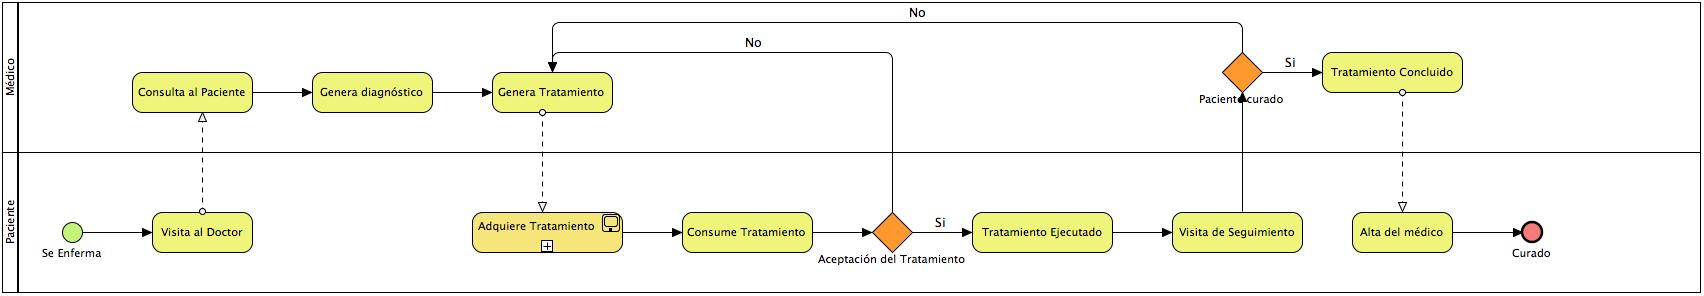
\includegraphics[width=1.1\textwidth]{images/cap2/Proceso1}
	\caption{Proceso médico en la actualidad} \label{fig:proceso1}
\end{figure}

\begin{figure}[htb]
	\centering
	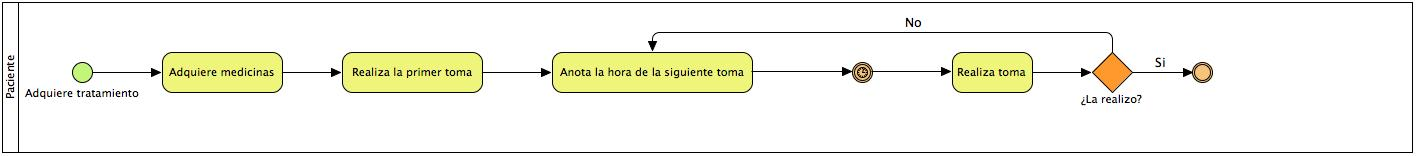
\includegraphics[width=1.1\textwidth]{images/cap2/AdquiereTratamientoP1}
	\caption{Sub-proceso Adquiere tratamiento en la actualidad} \label{fig:subproceso1}
\end{figure}

En cambio con el uso de la aplicación como se muestra en la imagen \ref{fig:proceso2} y su subproceso \ref{fig:subproceso2} podemos notar cómo el uso de las nuevas tecnologías ayuda tanto a los pacientes como a los médicos.

\begin{figure}[htb]
	\centering
	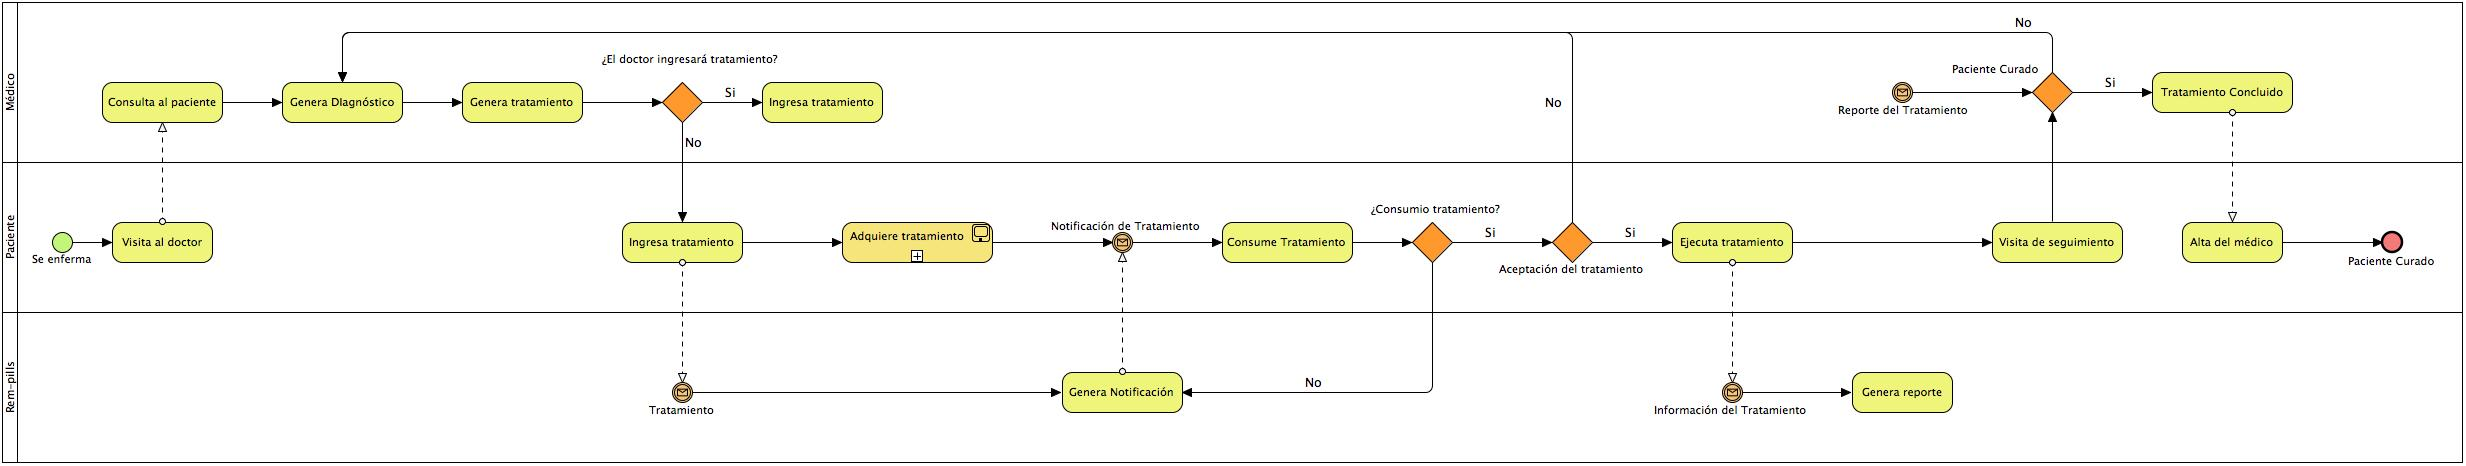
\includegraphics[width=1.1\textwidth]{images/cap2/Proceso2}
	\caption{Proceso médico con ayuda de la aplicación} \label{fig:proceso2}
\end{figure}

\begin{figure}[htb]
	\centering
	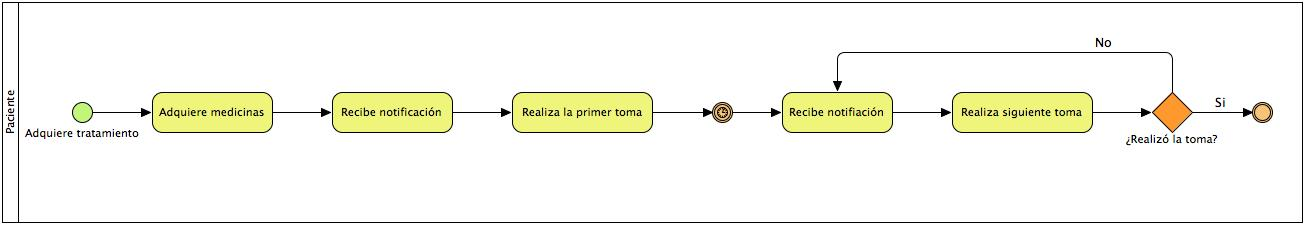
\includegraphics[width=1.1\textwidth]{images/cap2/AdquiereTratamientoP2}
	\caption{Sub-proceso Adquiere tratamiento con ayuda de la aplicación} \label{fig:subproceso2}
\end{figure}



\section{Casos de uso}
En el análisis realizado para la aplicación Rem-Pills se identificaron los siguientes casos de uso como se muestra en la figura\ref{fig:casosdeuso}.

\begin{figure}[htb]
	\centering
	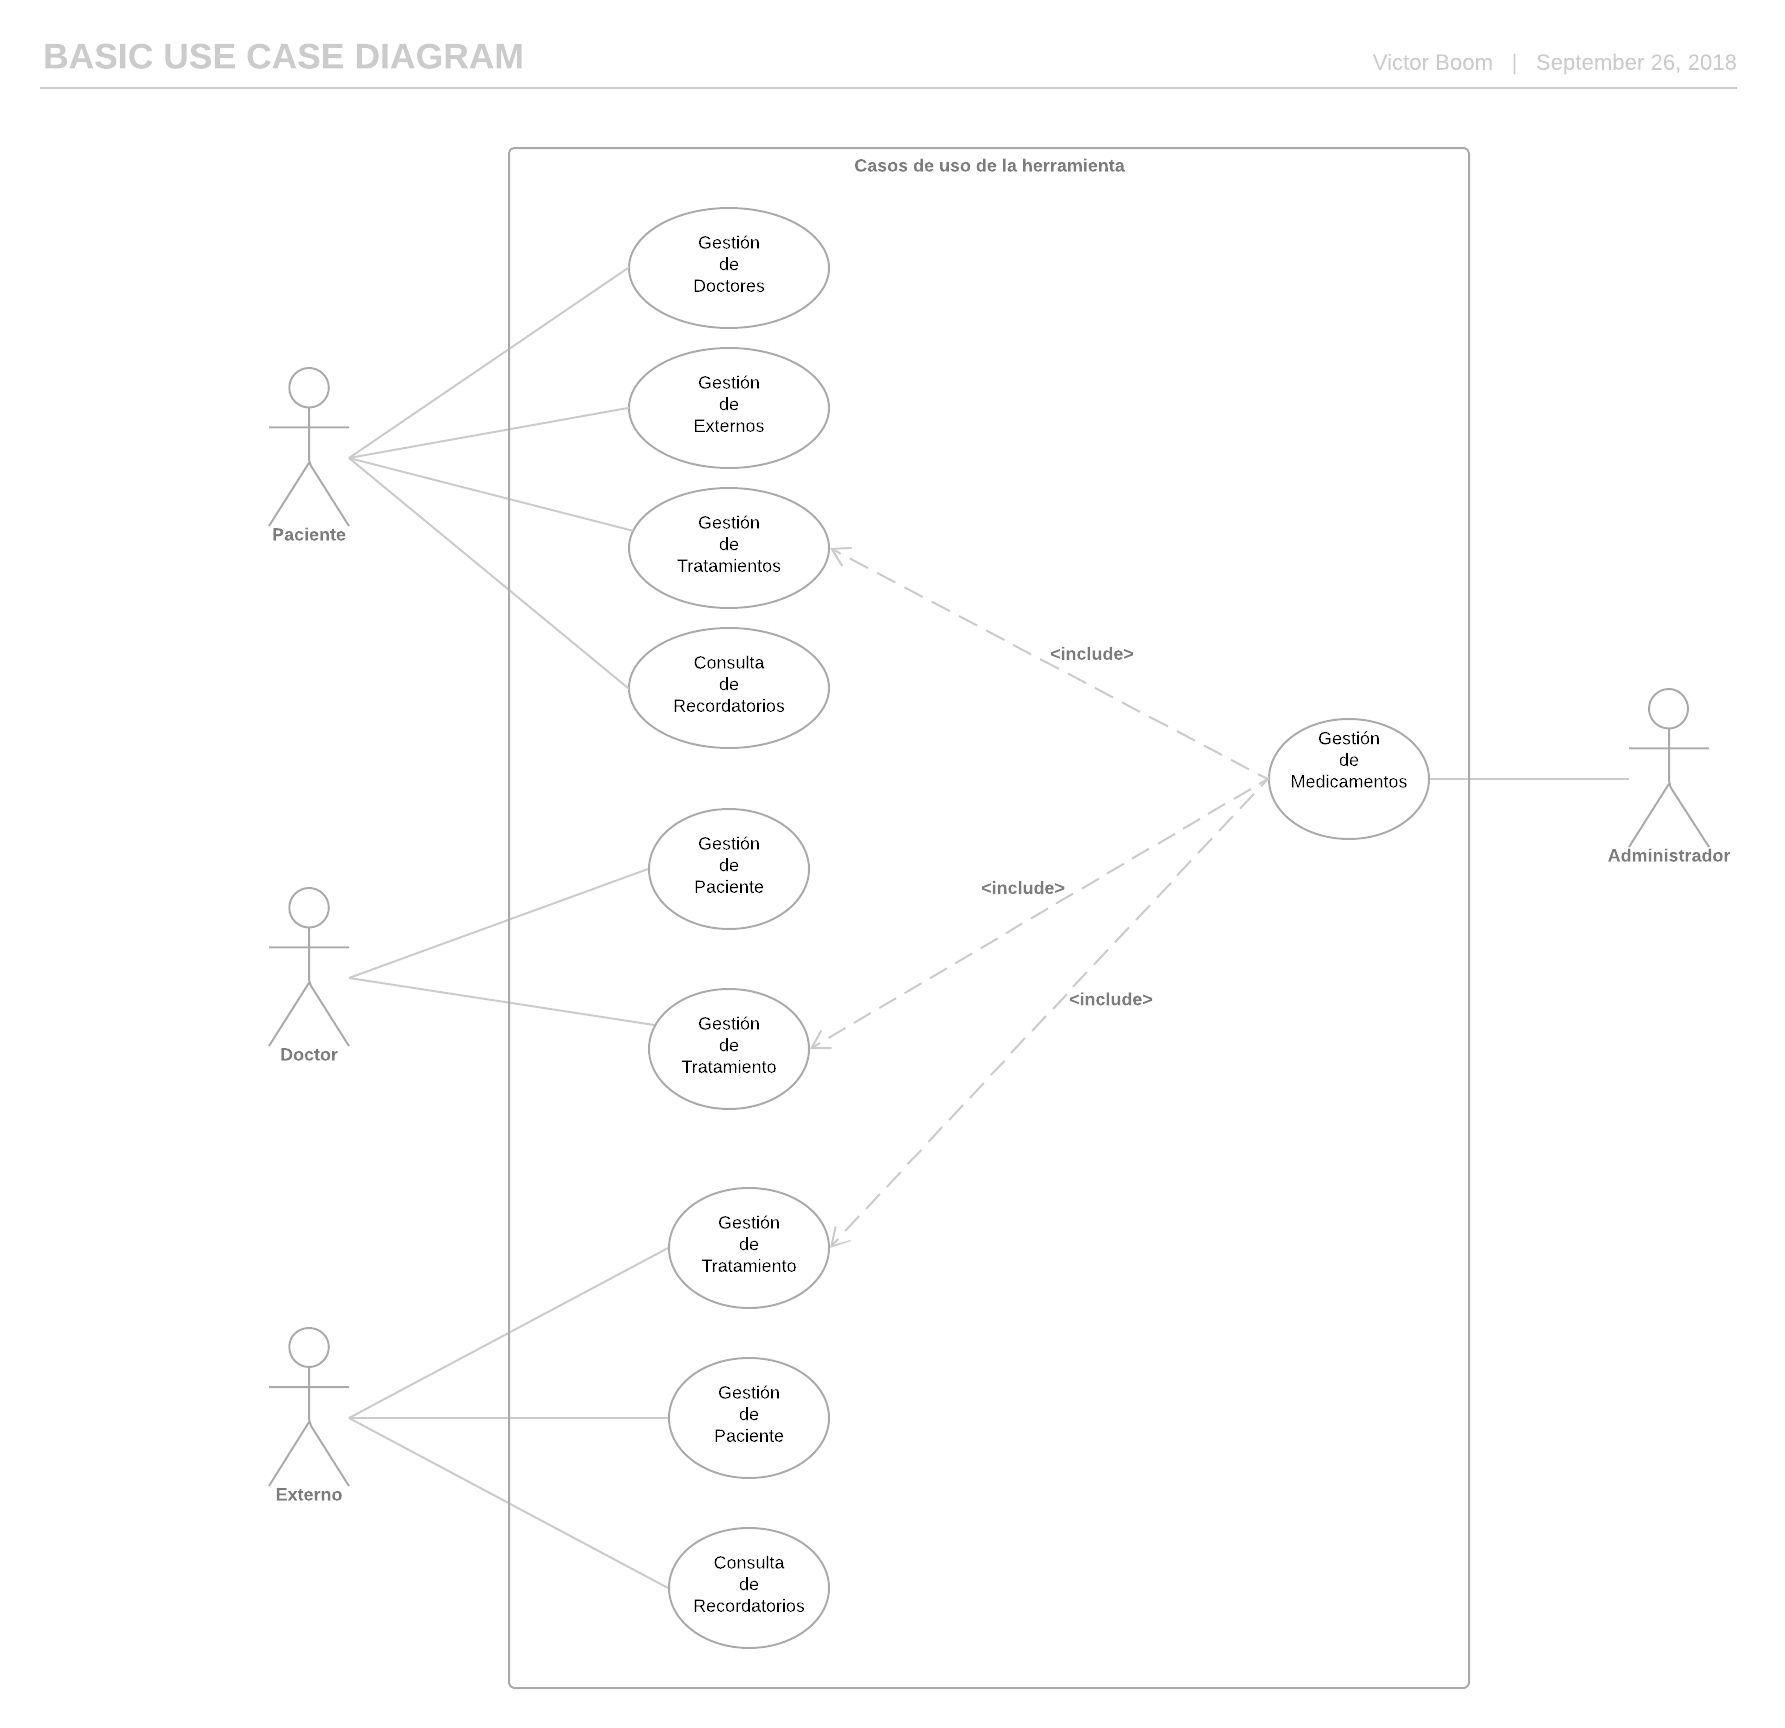
\includegraphics[width=0.7\textwidth]{images/cap2/casosdeuso}
	\caption{Casos de uso del paciente} \label{fig:casosdeuso}
\end{figure} 



La aplicación cuenta con los siguientes casos de uso:
\begin{itemize}
	\item Paciente:
		\begin{itemize}
			\item CUP1: Iniciar Sesión.
			\item CUP2: Recuperar Contraseña.
			\item CUP3: Registro de Cuenta.
			\item CUP4: Consultar Datos Personales.
			\item CUP5: Editar Datos Personales.
			\item CUP6: Cambiar Contraseña
			\item CUP7: Consultar Tratamiento.
			\item CUP8: Consultar Información de Tratamiento.
			\item CUP9: Editar Tratamiento.
			\item CUP10: Agregar Tratamiento.
			\item CUP11: Agregar Medicamento.
			\item CUP12: Agregar Doctor.
			\item CUP13: Editar Doctor.
			\item CUP14: Eliminar Doctor.
			\item CUP15: Consultar Doctor.
			\item CUP16: Recibir Notificación.
			\item CUP17: Mandar Alerta.
			\item CUP18: Consultar Recordatorios.
			\item CUP19: Consultar Alertas.
			\item CUP20: Agregar Auxiliar.
			\item CUP21: Editar Auxiliar.
			\item CUP22: Consultar Auxiliar
			\item CUP23: Eliminar Auxiliar.
			\item CUP24: Agregar Contacto de Emergencia.
			\item CUP25: Editar Contacto de Emergencia.
			\item CUP26: Consultar Contacto de Emergencia.
			\item CUP27: Eliminar Contacto de Emergencia.
		\end{itemize}
%	\item Doctor:
%		\begin{itemize}
%			\item 
%		\end{itemize}
%	\item Auxiliar:
	
\end{itemize}
%\begin{itemize}
%	
%	\item Gestión de Doctores:
%		\begin{itemize}
%			\item Agregar Doctor: Este caso de uso permitirá a un paciente agregar a un doctor.
%			\item Eliminar Doctor: Este caso de uso permitirá a un paciente a eliminar a un doctor.
%			\item Consultar Doctor: Este caso de uso permitirá a un paciente a consultar información relevante de su doctor.
%		\end{itemize}
%	Como se puede notar el caso de uso \textbf{Gestión de Doctores} engloba tres tipos de casos de uso distintos.
%	
%	\item Gestión de Auxiliares:
%	\begin{itemize}
%		\item Agregar Auxiliar: Este caso de uso permitirá a un paciente agregar a un auxiliar.
%		\item Eliminar Auxiliar: Este caso de uso permitirá a un paciente a eliminar a un auxiliar.
%		\item Consultar Axiliar: Este caso de uso permitirá a un paciente a consultar información relevante de su auxiliar.
%	\end{itemize}
%	Como se puede notar el caso de uso \textbf{Gestión de Auxiliar} engloba tres tipos de casos de uso distintos.
%	
%	\item Gestión de Pacientes:
%	\begin{itemize}
%		\item Agregar Paciente: Este caso de uso permitirá a un doctor y a un auxiliar agregar a un doctor.
%		\item Eliminar Paciente: Este caso de uso permitirá a un doctor y a un auxiliar a eliminar a un doctor.
%		\item Consultar Paciente: Este caso de uso permitirá a un un doctor y a un auxiliar a consultar información relevante de su doctor.
%	\end{itemize}
%	Como se puede notar el caso de uso \textbf{Gestión de Pacientes} engloba tres tipos de casos de uso distintos.
%	
%	\item Gestión de Tratamientos: 
%	\begin{itemize}
%		\item Agregar Tratamiento: Este caso de uso permite tanto al paciente, doctor y auxiliar agregar un tratamiento.
%		\item Eliminar Tratamiento: Este caso de uso permite tanto al paciente, doctor, y auxiliar eliminar un tratamiento existente.
%		\item Consultar Tratamiento: Este caso de uso permite tanto al paciente, doctor y auxiliar consultar un tratamiento existente.
%		\item Editar Tratamiento: Este caso de uso permite tanto al paciente, doctor, y auxiliar editar un tratamiento existente.
%	\end{itemize}
%	
%	\item Gestión de Recordatorios:
%	\begin{itemize}
%		\item Editar recordatorio
%		\item Consultar recordatorio
%	\end{itemize}
%	
%	\item Gestión de Medicamentos:
%	\begin{itemize}
%		\item Agregar medicamento:
%		\item Eliminar medicamento:
%		\item Editar medicamento:
%		\item Consultar medicamento:
%	\end{itemize}
%\end{itemize}
